\section{Background and Related Work}\label{sec:aslevel:background}

This section describes background of this chapter and presents related work. We start with an overview on measurement studies of live BitTorrent networks and show different approaches to reduce inter-ISP traffic discussed in the ALTO working group of the IETF. Finally, we introduce studies that infer the inter-AS relations based on BGP routing information.
We briefly describe the structure of the YouTube video CDN and give a short introduction in the principles of crowdsourcing.
Further, we summarize related work in the field of distributed active measurements of CDNs as well as work related to crowdsourcing aided network measurements.

\subsection{Measurements and Models of Live BitTorrent Networks}

BitTorrent is a peer-to-peer file-sharing protocol, which is based on multi-source downloads between the users. All the users, i.e., \textit{peers}, sharing the same file belong to a \textit{swarm}, c.f., \reffig{fig:aslevel:p2p}. To join the swarm, a peer requests addresses of other peers at an index server called \textit{tracker}. In the standard BitTorrent algorithm the tracker uses random peer selection to select a subset of peers that are in the swarm. Then, the joining peer tries to establish a neighbor relation to the peers it got from the tracker and collects all peers which accepted the request in his \textit{neighbor} set. The peer signals interest to all neighbors which have parts of the file it still needs to download. To which neighbor a peer is willing to upload data is decided by the choking algorithm, which is explained in \cite{cohen:bt}.

As basis of our methodology for modeling inter-ISP BitTorrent traffic, the results in \cite{Hossfeld2011} are revisited. In \cite{Hossfeld2011} the authors provide measurements of a large number of live BitTorrent swarms taken from popular index servers such as \emph{The Pirate Bay}, \emph{Mininova}, and \emph{Demonoid}. Using the IP addresses of the peers, the authors associate every peer with its AS and estimate the potential of ALTO mechanisms based on the differentiation between local peers (peers in the same AS) and remote peers located in other ASes. In contrast, we consider the actual Internet topology in this work, i.e., the inter-ISP relations, the ISP classification in the Internet hierarchy, and the AS paths between the peers in order to estimate the optimization potential of ALTO mechanisms.

The authors of \cite{Kryczka2011} use the peer exchange protocol (PEX) in order to measure the neighbor set of all peers participating in a number of live BitTorrent swarms. Based on this information, they model the graph topology of the swarms and compare the structure to random graphs. They also investigate clustering of peers within ASes and countries, but do not focus on inter-AS relations and AS paths between peers as we do in this work.

In addition, there are measurement studies that examine and model distinct features of BitTorrent networks. In \cite{Izal2004}, a single swarm was measured for five months with a focus on the download times of the peers. Additional parameters such as the peer inter-arrival times in the swarm, their upload capacity and their online time are considered in \cite{Pouwelse2005}. The authors of \cite{Guo2005} investigate these parameters also in multi-swarm scenarios. Finally, \cite{Zhang2010} measures \unit[4.6]{million} torrents to provide an overview of the entire BitTorrent ecosystem with its different communities and index servers. Our study differs from these works in that it focuses on the location of the peers in the Internet and the AS paths between the peers.

% \subsection{ALTO Mechanisms and Their Performance Evaluation}
%
% Various mechanisms to reduce the inter-ISP traffic generated by BitTorrent and other P2P applications are currently being investigated. Besides caching of BitTorrent traffic \cite{Lehrieder2010a,Lehrieder2012,Pacifici2012}, which might involve legal issues, changing standard BitTorrent algorithms is a promising approach. The authors of \cite{Aggarwal2007} propose to use an oracle service provided by the ISP guiding the peers in their peer selection process. The evaluation uses a Gnutella network and shows that intra-AS traffic is increased significantly without a negative impact on the overlay graph. Similar approaches are proposed for BitTorrent. Bindal et al. \cite{Bindal2006} reduce the inter-ISP traffic by modifying the neighbor set of the BitTorrent peers, which can be done at the tracker or enforced by the ISPs using deep packet inspection. Their simulations use a uniform peer distribution over ASes and show a high optimization potential of this approach. The authors of \cite{Xie2008} propose to use \emph{iTrackers} to guide the peers and formulates an optimization problem to find the best neighbor sets. Finally, Oechsner et al. \cite{Oechsner2009} propose to change the choke algorithm of BitTorrent to further reduce inter-ISP traffic and evaluate it via simulations in homogeneous scenarios. The BitTorrent plugin \emph{Ono} \cite{Choffnes2008} uses the servers of content distribution networks (CDN) as landmarks and estimates the proximity of two peers by the similarity of the CDN re-direction behavior.
%
% The authors of \cite{gkantsidis2006planet} investigate analytically the capabilities of a P2P-based content distribution network and the impact of locality. In contrast to our work, they use traffic characteristics which arise from software updates and do not consider AS relationships.
% A set of evaluations of ALTO mechanisms uses scenarios inspired by measurements of live BitTorrent swarms \cite{Cuevas2011,Blond2011,Lehrieder2011}. The studied scenarios consider heterogeneous peer distributions where some ASes contain more peers of a specific swarm than others. Nevertheless, they do not take into account inter-AS relations and the AS paths between two peers. This is different in our study. Using the AS affiliation of peers and the data obtained from Caida.org, we infer the actual paths of the BitTorrent connections in the Internet. In addition, we focus on the inter-ISP relations and investigate to which degree selfish ISPs profit from recommending their peers to preferentially use connections to peers located in lower tier ASes.

\begin{figure}[bt]
	\centering
\vspace{-0.2cm}
\hspace{-0.5cm}
	\begin{subfigure}[b]{0.54\textwidth}
	  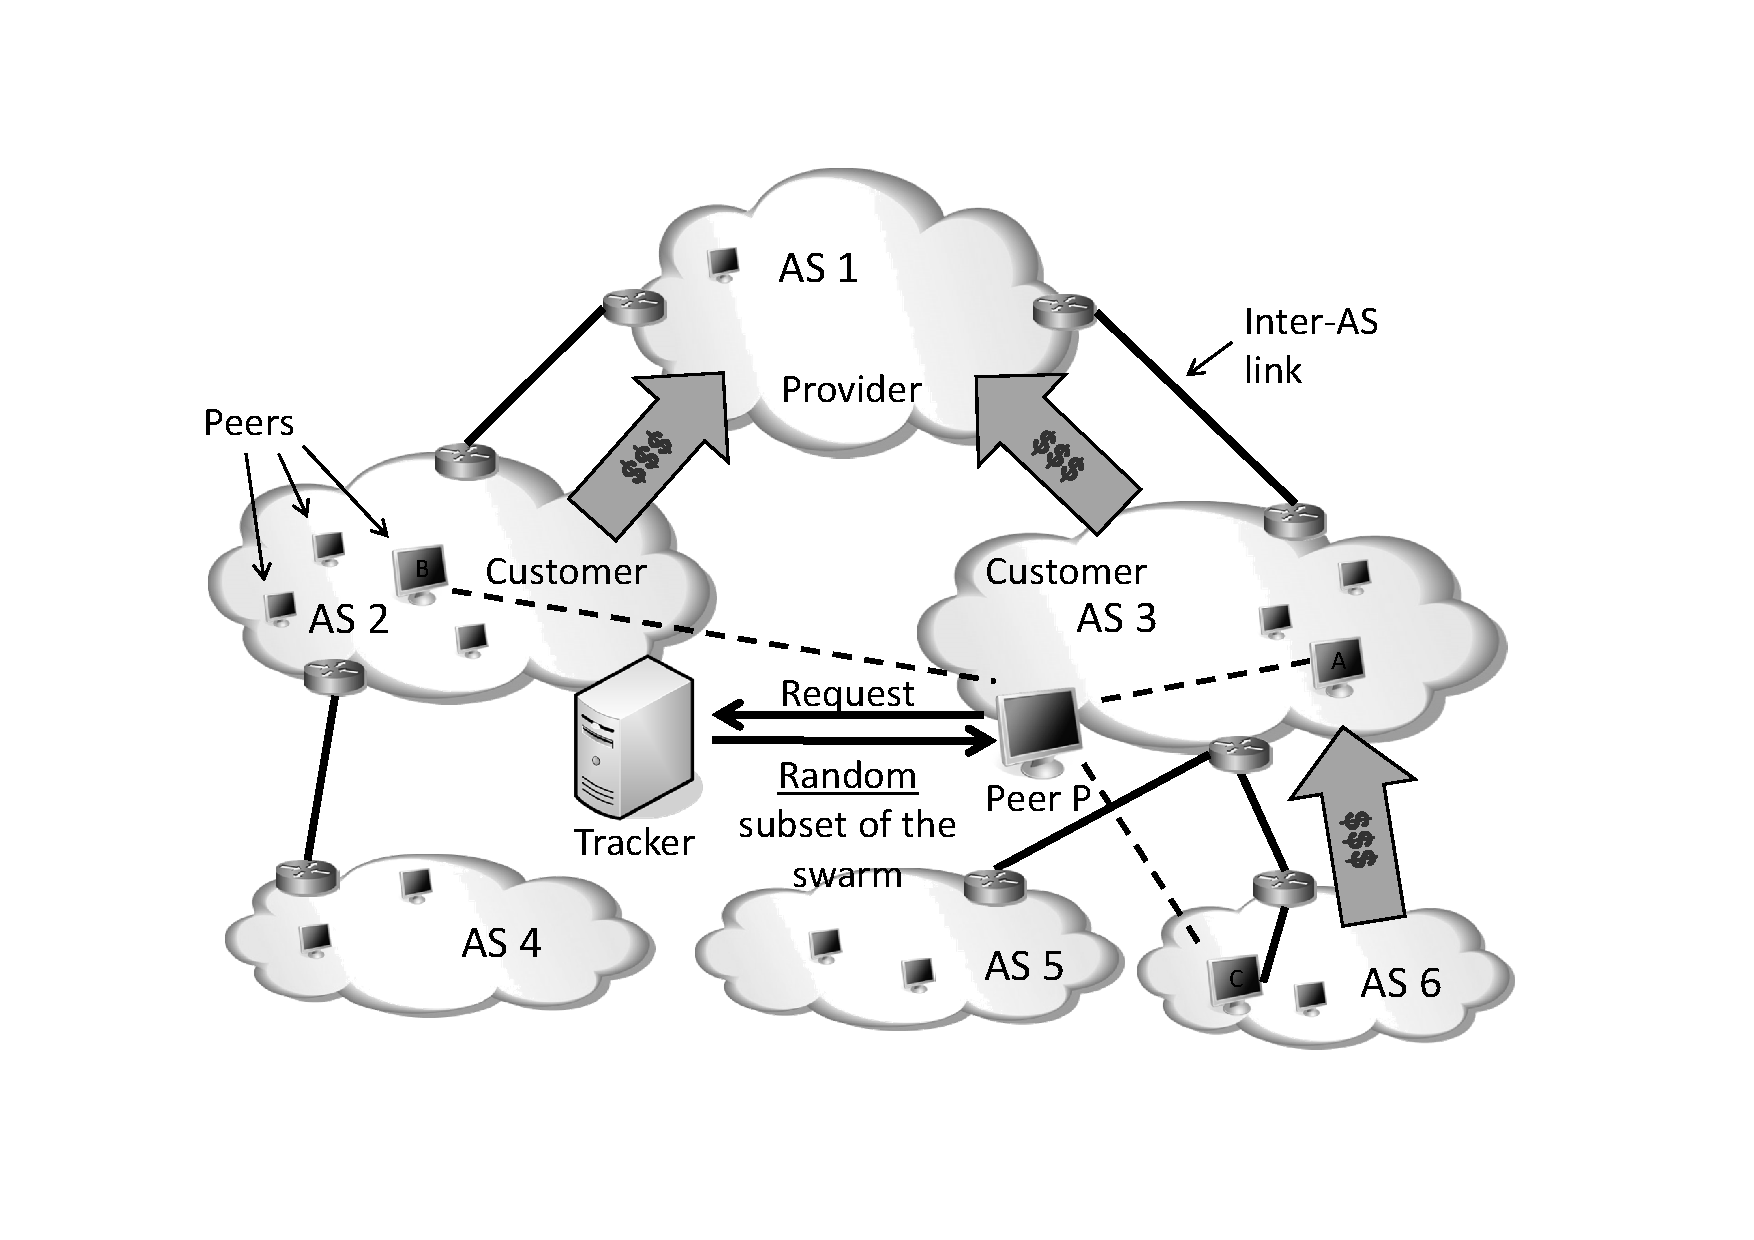
\includegraphics[width=\textwidth]{aslevel/figs/p2p}
    \vspace{-0.5cm}
    \caption{Peer-to-peer}
    \label{fig:aslevel:p2p}
  \end{subfigure}
\hspace{-0.5cm}
	\begin{subfigure}[b]{0.54\textwidth}
	 	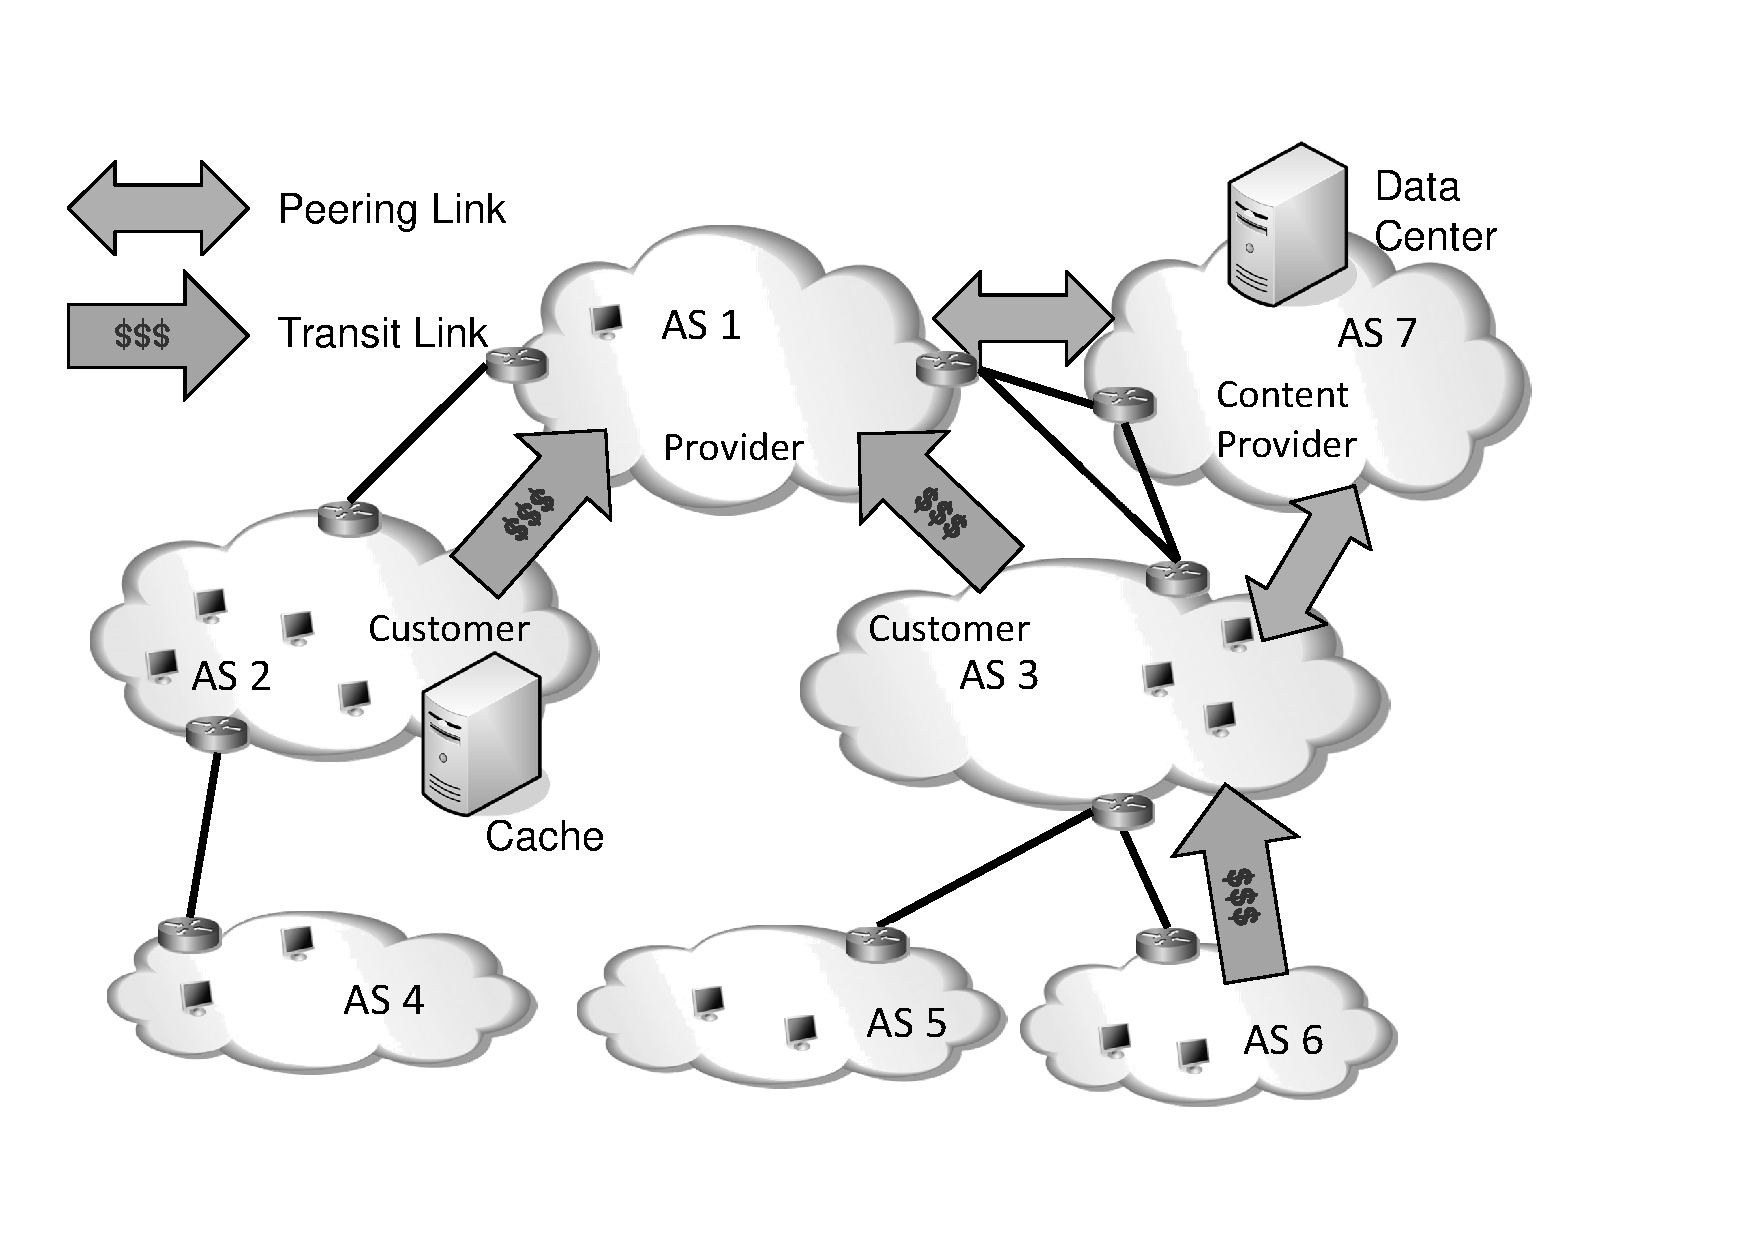
\includegraphics[width=\textwidth]{aslevel/figs/cdn}
    \vspace{-0.5cm}
    \caption{Content delivery network}
    \label{fig:aslevel:cdn}
	\end{subfigure}
\hspace{-0.5cm}
	\caption{Autonomous system topology with a peer-to-peer (left) and a content delivery network (right).}\label{fig:aslevel:p2pcdn}
\end{figure}

\subsection{Measurements of AS Relations and Topologies}

Autonomous systems are individual parts of the Internet, which are operated by ISPs.
On a technical level, the traffic exchange between the ASes is controlled by the Border Gateway Protocol (BGP)\cite{trangia2009}. However, commercial relations between ISPs determine the routing policies configured via BGP.
%The traffic exchanged between autonomous systems is inter-domain traffic. It is differentiated from intra-domain traffic, which is the traffic in the autonomous system.
An ISP must buy transit services to access parts of the Internet it neither owns nor can access by its customers.
Hence, to route traffic between autonomous systems ISPs engage in business relationships.
These business relationships are usually not open for public but they can be abstracted into three common types \cite{gao2001}.
The relationship between two ASes can be customer-to-provider (c2p), peer-to-peer (p2p) or sibling-to-sibling (s2s), c.f., \reffig{fig:aslevel:p2pcdn}.
A customer-to-provider link is present if the customer AS pays the provider AS for transit service, i.e., the provider forwards the traffic of the customer and its customers. In a peer-to-peer relation the ASes have an agreement that they exchange each others traffic and the traffic of their customers, without paying each other. Sibling-to-sibling are links between ASes of the same organization. These relations are defined in business agreements and kept secret, but they can be inferred by analyzing the routing between autonomous systems.

The approach that is most widely used to infer AS relationships is analyzing BGP routing tables. The data set used in this work is also produced by inferring BGP tables as described in \cite{dimitropoulos2007relationships}. Therefore, AS links are extracted from RouteViews BGP tables. First sibling-to-sibling links are identified by looking up organizations that own multiple AS numbers. Then customer-to-provider relationships are inferred by a heuristic that is based on the idea of relaxing the requirement for a maximal number of valid paths and using the AS degree information to detect paths that are invalid. Most challenging is the inference of peer-to-peer links since paths remain valid if peer-to-peer links are replaced by a customer-to-provider or provider-to-customer link. The authors of \cite{dimitropoulos2007relationships} develop a heuristic which combines the strengths of previous approaches by \cite{gao2001} and \cite{di2003computing}. The inferred relationships were validated by surveys, showing that \unit[96.5]{\%} customer-to-provider, \unit[82.8]{\%} peer-to-peer, and \unit[90.3]{\%} sibling-to-sibling of the inferred relationships are correct.

\subsection{Evolution and Structure of Content Delivery Networks}
%To understand why distributed measurements are necessary and to provide the basic ideas of content delivery network structures, we briefly describe the evolution of content delivery networks and the functionality of the YouTube CDN.
Since the launch of the YouTube service content delivery has drastically changed.
While the amount of traffic transported over peer-to-peer networks remained about the same, the traffic transported by content delivery networks has increased exponentially \cite{cisco2016}.
The number of users watching videos on demand has massively increased and the bandwidth to access videos is much higher.
Furthermore, the increased bandwidth enables web services to be interactive by using dynamic server- or client-side scripts.
The appearance of dynamic services and the increasing quality of multimedia content raised user expectations and the demand on the servers.
To bring content in high quality to end-users with low latency and to deal with increasing demand, content providers have to replicate and distribute the content to get it close to end-users.
Thus, content delivery networks such as the Google CDN evolved.

The global expansion of the CDNs also changes the structure of the Internet.
Google has set up a global backbone which interconnects Google's data centers to important edge points of presence.
Since these points of presence are distributed across the globe, Google can offer direct peering links to access networks with many end users, c.f. \reffig{fig:aslevel:cdn}.
Such, access network providers save transit costs, while Google is able to offer services with low latency.
To bring content even closer to users ISPs can deploy Google servers inside their own network to serve popular content, including YouTube videos~\cite{gcc}.

To select the closest server for a content request and to implement load balancing CDNs use the Domain Name System (DNS).
Typically a user watches a YouTube video by visiting a YouTube video URL with a web browser.
The browser then contacts the local DNS server to resolve the hostname.
Thereafter, the HTTP request is directed to a front end web server that returns an HTML page including URLs for default and fallback video servers.
These URLs are again resolved by DNS servers to physical video servers, which stream the content.
The last DNS resolution can happen repeatedly until a server with enough capacity is found to serve the request.
Thus, load balancing between the servers is achieved~\cite{adhikari2012vivisecting}.

\subsection{Crowdsourcing}
Crowdsourcing is an emerging service in the Internet that enables outsourcing jobs to a large, anonymous crowd of users~\cite{articles2013-113}.
So called \emph{Crowdsourcing platforms} act as mediator between the users submitting the tasks, the \emph{employers}, and the users willing to complete these tasks, the \emph{workers}.
All interactions between workers and employers are usually managed through these platforms and no direct communication exits, resulting in a very loose worker-employer relationship.
The complexity of Crowdsourcing tasks varies between simple transcriptions of single words~\cite{vonAhn2008} and even research and development tasks~\cite{innocentive}.
Usually, the task description are much more fine granular than in comparable forms in traditional work organization~\cite{conf2011-417}.
This small task granularity hold in particular for \emph{micro-tasks}, which can be completed within a few seconds to a few minutes.
These tasks are usually highly repetitive, e.g., adding textual descriptions to pictures, and are grouped in larger units, so called \emph{campaigns}.

\subsection{Distributed Measurements of Content Delivery Networks}
There already exist a number of publications which study the structure of the YouTube CDN and its selection of video servers.
A distributed active measurement platform is necessary for these evaluation, because the CDN mechanisms consider the client locations, both geographical as well as in terms of the connected access network.
In \cite{torres2011dissecting} two university campus networks and three ISP networks were used to investigate the YouTube CDN from vantage points in three different countries.
The results show that locality in terms of latency is not the only factor for video server selection.

While the view of five different ISPs on a global CDN is still narrow, the authors of \cite{adhikari2011you} used PlanetLab to investigate the YouTube server selection strategies and load-balancing.
They find that YouTube massively deploys caches in many different locations worldwide, placing them at the edge of the Google autonomous system or even at ISP networks.
The work is enhanced in \cite{adhikari2012vivisecting}, where they uncover a detailed architecture of the YouTube CDN, showing a 3-tier physical video server hierarchy.
Furthermore, they identify a layered logical structure in the video server namespace, allowing YouTube to leverage the existing DNS system and the HTTP protocol.

However, to assess the expansion of the whole YouTube CDN and its cache locations in access networks, the PlanetLab platform, which is located solely in National Research and Education Networks~(NRENs), is not suitable, since it does not reflect the perspective of end users in ISP access networks.
Therefore, a different distributed measurement platform is used in \cite{rafetseder2011exploring} which runs on end user equipment and thus implies a higher diversity of nodes and reflects the perspective of end user in access networks.
However, the number of nodes that was available for the measurement is too small to obtain a global coverage of vantage points

To achieve both, the view of access networks and a high global coverage with a large number of measurement points, the participation of a large number of end users in the measurement is necessary.
Bischof et al. \cite{bischof2011crowdsourcing} implemented an approach to gather data form peer-to-peer networks to globally characterize the service quality of ISPs using volunteers.

In contrast to this we propose using a commercial crowdsourcing platform to recruit users running a specially designed measurement software and therewith act as measurement probes.
In comparison to other approaches using volunteers, this approach offers better scalability and controllability, because the number and origin of the participants can be adjusted using the recruiting mechanism of the crowdsourcing platform.
This is confirmed by Table~\ref{tab:CvsS} which compares a crowdsourcing study with a social network study quantitatively. The crowdsourcing study  is described in \cite{bookchapter2013-18}. The study is designed to assess the subjective QoE for multimedia applications, like video streaming.
The same study was conducted additionally in a social network environment for recruiting test users.
Table~\ref{tab:CvsS} shows that acquiring people in crowdsourcing platforms takes very short time compared to asking volunteers in a social network, which allows adding participants easily.
Furthermore, the completion time of the campaign of 31 hours is much shorter compared to the 26 days for the social network campaign.
Finally, in the crowdsourcing campaign workers can be selected according to their country, which allows distributing the campaign on many different countries. In the social network the coverage of countries depends on the network of user groups, which spread the campaign.
Hence, it is easy to control the number and origin of subjects participating in a crowdsourcing campaign and the completion time is considerably fast, which makes the campaign scalable and controllable. The price you pay is the reward for the workers that summed up to a total of 16 Euro for that campaign.

\begin{table}[tb]
\caption{Quantitative Comparison: Crowdsourcing / Social Network Study.} \label{tab:CvsS}
\begin{center}
{\footnotesize
	\begin{tabular}{|p{.29\textwidth}|p{.29\textwidth}|p{.29\textwidth}|} \hline
		\textbf{} & \textbf{Crowdsourcing (C)} & \textbf{Social network (S)} \\ \hline
		\textbf{Implementation time} & about 2 weeks; test implemented via dynamic web pages, application monitoring & same as for (C) \\ \hline
		\textbf{Time for acquiring people} & 5 minutes & 2 hours, as users (groups) were asked individually \\ \hline
		\textbf{Campaign submission cost} & 16 Euro & 0 Euro \\ \hline
		\textbf{Subject’s reward} & 0.15 Euro & 0 Euro \\ \hline
		\textbf{Number of test conditions} & 3 & 3 \\ \hline
		\textbf{Advertised  people} & 100 & 350 \\ \hline
		\textbf{Campaign completion time} & 31 hours & 26 days; strongly depends on advertised user groups however \\ \hline
		\textbf{Participating users} & 100 & 95 \\ \hline
		\textbf{Reliable users (very strict filtering of users)} & 30 & 58 \\ \hline
		\textbf{Number of different countries of subjects} & 30 & 3; strongly depends on users groups however \\ \hline
		\end{tabular}
}
\end{center}
\end{table}



The Internet Census Dataset was validated forensically in \cite{dainotticaida}.
In \cite{krenc2014internet} the scope of the dataset is taken into perspective and show that, although there are some qualitative problems, the measurement data seems to be authentic.
We use the Internet Census Dataset to determine the number of active IP-addresses for each autonomous system in the Internet.
%To the best of our knowledge, this is the first work which evaluates a gl
%To the best of our knowledge this is the first work which uses crowdsourcing for a distributed active measurement platform.
